\documentclass[a4paper]{article}

\usepackage{draftwatermark}
\usepackage{algorithm2e}
\usepackage{paralist}
\usepackage{graphicx}
\usepackage{authblk}
\usepackage{amsmath}
\usepackage{wrapfig}
\usepackage{amsthm}

% TODO replace 21 with 22
% TODO remove this in the final version
\newcommand{\keyword}[1]{\textbf{#1}}

\newcounter{main}
\newtheorem{prop}[main]{Proposition}
\newtheorem{comp}[main]{Computation}
\newtheorem{cor}[main]{Corollary}
\newtheorem{thm}[main]{Theorem}
\newtheorem{lem}[main]{Lemma}
\newtheorem{fact}[main]{Fact}
\theoremstyle{definition}
\newtheorem{dfn}[main]{Definition}
\newtheorem*{spin}{SPIN Axiom \cite{ck09}}
\theoremstyle{remark}
\newtheorem{rem}[main]{Remark}

\title{A Kochen-Specker system has at least 21 vertices\\
        {\small (extended abstract)}}

\author{Sander Uijlen}
\author{Bas Westerbaan}

% TODO will we keep these @cs.ru.nl addresses?
\affil{{\small Institute for Computing and Information Sciences\\
        Radboud Universiteit Nijmegen}\\
   \{\texttt{suijlen},\texttt{bwesterb}\}\texttt{@cs.ru.nl}}

\begin{document}

\maketitle

\begin{abstract}
    At the heart of the Conway's Free Will theorems and Kochen and Specker's
        argument against noncontextual hidden variable theories
    is the existence of a Kochen-Specker (KS) system:
    a set of points on the sphere,
    that has no~$\{0,1\}$-coloring such that
    at most one of two orthogonal points are colored~$1$
    and of three pairwise orthogonal points exactly one
    is colored~$1$.
    In public lectures, Conway encouraged the search for small
    KS systems.  
    At the time of writing, the smallest known
    KS system has 31 vectors.  

    Arends, Ouaknine and Wampler have shown that a KS system has at least
    18 vectors, by reducing the problem to the existence of graphs
    with a topological embeddability and non-colorability property.
    Deciding embeddability and the sheer number of graphs on more than~$17$
    vertices, proved the bottleneck in their search.

    Continuing their effort, we prove a restriction on the class of graphs
    we need to consider and develop a more practical decision procedure for
    embeddability to improve the lower bound to 21.
\end{abstract}
    
\section{Introduction}

% TODO whose idea is this orthogonality graph
\subsection{The experiment}

% TODO correct description of experiment
Consider the following experiment.  Shoot a deuterium atom,
or any other spin-1 particle,
along, say: the x-axis, through a inhomogeneous magnetic field.
Depending on the direction of the magnetic field,
the particle will move undisturbed
or deviate.

Quantum Mechanics only predicts the probability, given the configuration
of the field, whether the particle will deviate.
Its probabilistic prediction has been thoroughly tested.
One wonders: is there a deterministic noncontextual theory predicting the
outcome of this experiment?

Kochen and Specker proved that such a theory cannot satisfy:
% TODO note contextuality
\begin{spin}
    Given three pairwise orthogonal directions.
    In exactly one of the directions, the particle will not deviate.
\end{spin}
Their argument is based on the existence of a Kochen-Specker system.
\begin{dfn}
    A \keyword{Kochen-Specker (KS) system} is
    a finite set of points on the sphere
    for which each pair is not antipodal and
    there is no~\keyword{010-coloring}.
    A $010$-coloring is a~$\{0,1\}$-coloring of the points such that
        \footnote{
                In other papers, like \cite{aow11},
                the~$0$ and~$1$ are swapped, they consider 101-colorings.
                These colorings are of course equivalent and the difference
                arises from considering either squared spin measurements $S^2$, or $1-S^2$.
                %Then the colors correspond directly to the squared measurement
               	%outcome of the spin.
               	}
    \begin{enumerate}
        \item
            no pair of orthogonal points are both colored~$1$ and
        \item
            of three pairwise orthogonal points exactly one is colored~$1$;
            or alternatively: they are colored~$0$, $1$ and~$0$ in some order.
    \end{enumerate}
\end{dfn}
% TODO shorten this proof.
A point on the sphere obviously corresponds to a direction in space.
Because of this, the term point, vector and direction
can be used interchangeably. Antipodal points correspond to opposite
vectors and these span the same direction in space.

Suppose there is a KS system and a noncontextual deterministic theory satisfying
the SPIN Axiom.
Then we color a point of this system~$0$,
whenever this theory predicts that the particle will deviate
if the spin is measured in the direction corresponding to that point, and~$1$ otherwise.
Given two orthogonal points of the system,
we can find a third point orthogonal to both of them.
The SPIN axiom implies exactly one of them is colored~$1$, so they cannot both be colored~$1$.
Similarly, given three pairwise orthogonal vectors in the system,
the SPIN axiom implies exactly one of them is colored~$1$.
Hence there would be a 010-coloring of the KS system, quod non. Therefore a deterministic noncontextual theory cannot satisfy the SPIN Axiom.\\

The KS system proposed by Kochen and Specker contained 117 points\cite{ks}.
Penrose and Peres\cite{peres} independently found a smaller system of 33 points.
The current record is the 31 point system of Conway\cite[p.~197]{qtcm}.
As pointed out by \cite{c00,aow11}, finding small KS systems
is of both theoretical and practical interest.
In public lectures, Conway himself, stressed the search for small KS systems.

% TODO refer to non-3d systems
\subsection{Overview}
In \cite{aow11} Arends, Ouaknine and Wampler (AOW) give a computer aided proof
that a KS system must have at least 18 vectors.  We improve their lower bound
and show that a KS system must have at least 21 vectors.

First, in Subsection~\ref{sec:ksgraphs},
we repeat a part of AOW's work, in particular the reduction of
KS systems to graphs.
The bottleneck of their search was the sheer number of graphs
and the deciding whether such graphs are embeddable.

In Section~\ref{sec:ilb},
we improve upon their reduction,
to cut down the number of graphs to consider drastically,
and state the results of our main computation.
Finally, in Section~\ref{sec:emb},
we describe our practical embeddability test.

\subsection{Kochen-Specker graphs}
\label{sec:ksgraphs}
We follow \cite{aow11} and reduce the search for Kochen-Specker systems
to the search of a certain class of graphs.
First note that in a Kochen-Specker system we may replace a point with its
antipodal point.  They are both orthogonal to the same points and hence
the non-010-colorability is preserved.
Therefore, we may assume antipodal points are identified on the sphere.
That is: a Kochen-Specker system is a finite subset of the projective plane
that is not 010-colorable.
\begin{dfn}
Given a finite subset~$S$ of the projective plane
(or equivalently, of the northern hemisphere without equator).
Define its \keyword{orthogonality graph}~$G(S)$ as follows.
The vertices are the points of~$S$.
Two vertices are joined by an edge, if their corresponding points
are orthogonal.
\end{dfn}
\begin{dfn}
A graph~$G$ is called~\keyword{embeddable},
if it occurs as a subgraph of an orthogonality graph;
that is: if there is a finite subset~$S$ of the projective plane,
such that~$G \leq G(S)$.
\end{dfn}
% TODO add remark on subgraph definition?
\begin{dfn}
A graph is~\keyword{010-colorable}
if there is a~$\{0,1\}$-coloring, such that
\begin{enumerate}
\item
for each triangle there is exactly one vertex that is colored~$1$ and
\item
adjacent vertices are not both colored~$1$.
\end{enumerate}
\end{dfn}
\begin{dfn}
A \keyword{Kochen-Specker graph}
is a embeddable graph that is not 010-colorable.
\end{dfn}
It is an easy, but important, consequence of the definitions that:
\begin{fact}
    A finite subset~$S$ of the projective plane
    is a Kochen-Specker system,
    if and only if its orthogonality graph~$G(S)$
    is Kochen-Specker.
\end{fact}
To prove there is no Kochen-Specker system on~$17$ points,
it would be sufficient to enumerate all graphs on~$17$ vertices
and check these are not 010-colorable or not embeddable.
However, this is infeasible as there are
already~${\sim}10^{26}$ non-isomorphic
graphs on~$17$ points.
% TODO OEIS A000088
Luckily, we can restrict ourselves to certain classes of graphs.
\begin{prop}[\cite{aow11}]
    An embeddable graph does not contain a square.
\end{prop}
\begin{proof}
    Given two non antipodal points~$a\neq b$.
    Consider the points orthogonal to~$a$.
    This is a great circle.
    The points orthognal to~$b$ is a different great circle.
    They intersect in precisely two antipodal points.
    Hence, if~$c$ and~$d$ are both orthogonal to~$a$ and~$b$,
    then~$c$ and~$d$ are equivalent.
    Therefore, an embeddable graph cannot contain a square.
\end{proof}
The squarefreeness is a considerable restriction.  There are
only~${\sim}10^{10}$ non-isomorphic squarefree graphs on~$17$ vertices.
We can restrict ourselves to connected graphs.
% TODO OEIS A006786
\begin{prop}[\cite{aow11}]\label{prop:ks-conn}
    A minimal Kochen-Specker graph is connected.
\end{prop}
\begin{proof}
    Suppose~$G$ is a non-connected Kochen-Specker graph.
    Then one of its components is not 010-colorable.
    As a subgraph of an embeddable graph, is embeddable,
    this component is embeddable as well.
    Hence it is a smaller connected Kochen-Specker graph.
\end{proof}
The gain, however, is small.
There are only~${\sim}10^9$ non-isomorphic squarefree graphs on~$17$
vertices that are not connected.
We have verified the main result of \cite{aow11}:
\begin{comp}
There is a unique non-010-colorable squarefree connected graph on~$17$ or less
vertices. It looks as follows TODO
It is not embeddable, see TODO, and hence a Kochen-Specker
system has at least 18 points.
\end{comp}

\section{An improved lower bound}
\label{sec:ilb}
Continuing the effort of Arends, Ouaknine and Wambler,
we consider another restriction.
\begin{prop}
    A minimal Kochen-Specker graph has minimal vertex-order three.
\end{prop}
\begin{proof}
    Given a Kochen-Specker graph~$G$.
    Suppose~$v$ is a vertex with order less than or equal~$2$.
    Let~$G'$ be~$G$ with~$v$ removed.
    Clearly~$G'$ is embeddable.
    Suppose~$G'$ is 010-colorable.
    Then we can extend the coloring to a coloring of~$G$ as follows.
    If~$v$ is adjacent to only one or no vertex,
    then we can color~$v$ with~$0$.
    Suppose~$v$ is adjacent to two vertices, say~$w$ and~$w'$.
    If one of~$w$ or~$w'$ is colored~$1$, we can color~$v$ with~$0$.
    If both~$w$ and~$w'$ are colored~$0$, we can color~$v$ with~$1$.
    This would imply~$G$ is 010-colorable, quod non.
    Therefore~$G'$ is a smaller
    Kochen-Specker graph, which contradicts minimality.
\end{proof}
There are only~${\sim}10^7$
squarefree non-isomorphic graphs on 17 vertices with minimal vertex order 3.
Even though Arends, Ouaknine and Wampler
note this restriction once,
surprisingly, they did not restrict their graph enumeration
to graphs with minimal vertex order 3.

We continue with a strengthening of Proposition~\ref{prop:ks-conn}.
\begin{prop}
A minimal Kochen-Specker graph is biconnected,
that is: removing any single edge leaves the graph connected.
\end{prop}
\begin{proof}
Suppose we have a connected but not biconnected graph~$G$.
Then we can decompose
this graph into its biconnected components.  A biconnected components
is a maximal subgraph that is biconnected.
We can consider the graph of biconnected components~$B(G)$:
two biconnected components are adjacent if there is an edge
between a vertex in one component and a vertex in the other.
Note that there can at most be one edge between 
the vertices of biconnected components.
$B(G)$~does not contain loops: if it would
then the union of the biconnected components in the graph,
would be itself biconnected.

Now consider a leaf~$A$ in the biconnected component graph~$B(G)$. That is, $A$ is a component which is only connected to one other component.
Let~$B$ be the union of the remaining biconnected components.
There is exactly one pair of vertices~$(a,b)$
such that~$a \in A$, $b \in B$ and $a$ is adjacent to~$b$.

Take any~$b_2 \in B$ with~$b_2 \neq b$.
By assumption~$b_2$ is not adjacent to~$a$.
Define~$G'$ to be the graph~$G$ extended with the edge~$(a,b_2)$.
Clearly, $G'$ is not~010-colorable.  We will show that~$G'$ is embeddable.

Consider an embedding of~$G$.
Observe that a rotation of all (points corresponding to) elements of~$A$
along the axis spanned
by (the point corresponding to)~$b$, preserves all relevant
orthogonality relations.

Rotate the vectors of the embedding
along~$b$ such that~$b_2$ becomes orthogonal to~$a$.
It could that there are elements~$a'$ in~$A$
and~$b'$ in~$B$ that are rotated onto the same point.
Then consider rotations of all elements of~$B$ along~$a$.
There are finitely many angles for which two elements will overlap.
Hence, there is a rotation of all elements of~$B$ along~$a$
such that~$A$ and~$B$ do not overlap.
Note that all existing orthogonality relations are preserved.

These two rotations yield a new set of points on the sphere,
that demonstrate~$G'$ is embeddable.
Therefore, in generating all relevant graphs, we find both $G$ and $G'$. Since they have the same order, we might as well ignore the graph $G$. This shows it is sufficient to consider only biconnected graphs.
\end{proof}
We believe a minimal KS graph is also triconnected.
Although these arguments are pleasing,
they are of little use:
% TODO Add argument or computation for {2,3}-connected
% TODO note that restricting to (bi/tri)-connected is a waste of time
% TODO add graph 
\begin{comp}
    There are five non-isomorphic minimal
    squarefree connected graphs
    with minimal vertex order 3 and they have 10 vertices.
\end{comp}
\begin{cor}
    Any unconnected
    squarefree graph with minimal vertex order 3
    has at least 20 vertices, for it has two connected components,
    each with at least 10 vertices.
\end{cor}

% TODO is core x years a proper expression?
Now, we can state our main computation, which took roughly a week
    on a 64-core Opteron 6276.
\begin{comp}
    Let~$C_n$ denote the number of non-010 colorable squarefree
    graphs with minimal vertex order 3 on~$n$ nodes.  Then:

    \begin{center}
    \begin{tabular}{l|lllll}
        $n$ & $\leq 16$
            & $17$
            & $18$
            & $19$
            & $20$ \\
        \hline
        $C_n$ & $0$
            & $1$
            & $2$
            & $19$
            & $441$
    \end{tabular}
    \end{center}

    All these 463 graphs are not embeddable.
    % TODO add reference
\end{comp}


\section{Embeddability}
\label{sec:emb}
\begin{wrapfigure}{r}{0.40\textwidth}
\begin{center}
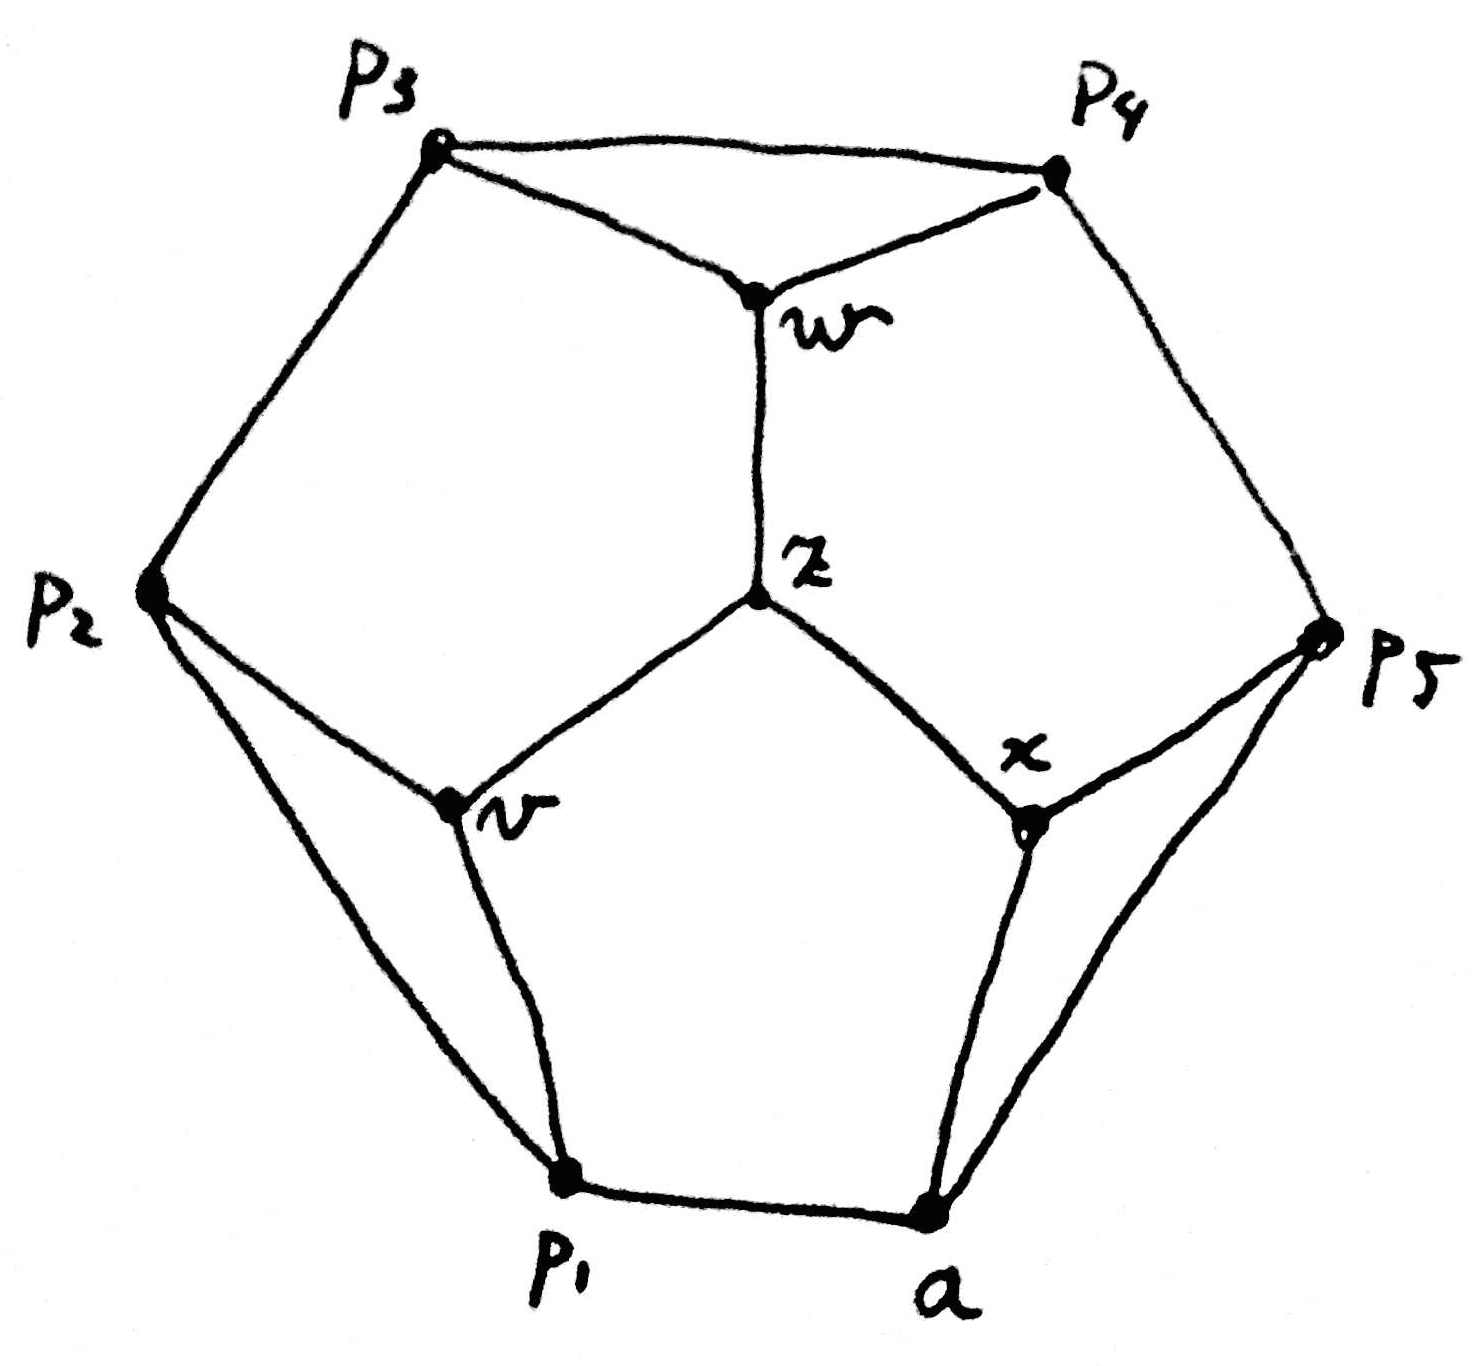
\includegraphics[width=50mm]{graphs/unemb-10-2.jpg}
\end{center}
\caption{One of the two minimal
        non-embeddable graphs
\label{fig:unemb-10-2}}
\end{wrapfigure}

Our computation has yielded a few hundred non-010-colorable graphs.
If we show one of them is embeddable, we have found a new KS system.
If we demonstrate all of them are not embeddable, we have
proven a lower bound on the size of a minimal KS system.

In~\cite{aow11}, Arends, Wampler and Ouaknine discuss several
computer-aided methods
to test embeddability of a graph.  None of these methods could decide
for all graphs considered, whether they were embeddable or not.
% TODO give a small description of their deficiencies
% TODO give intermediate computation.

We propose a new method,
which for all graphs we considered,
could decide
whether they were embeddable or not.
First we give a pen-and-paper example.
\begin{prop}\label{prop:unemb-10-2}
The graph in Figure~\ref{fig:unemb-10-2}
is not embeddable.
\end{prop}
\begin{proof}
Suppose it is embeddable.
Consider~$p_1$.
It is orthogonal to both~$a$ and~$v$.
$a$ and~$v$ are not collinear,
hence~$p_1$ must be collinear to~$v \times a$,
the cross-product of~$v$ and~$a$.
Similarly, $p_2$ is collinear to~$v \times p_1 = v \times (v \times a)$.
Continuing in this fashion,
we see that
\begin{equation}\label{eq:ue1}
    a \text{ is collinear to }
    x \times (x \times( w \times (w\times (v \times (v \times a))))).
\end{equation}
Now, we may assume that~$z=(0,0,1)$ and $x=(1,0,0)$.
Thus: $v=(v_1,v_2,0)$;
$w = (w_1,w_2,0)$
and $a = (0, a_2,a_3)$ for some~$-1 < v_1,v_2,w_1,w_2,a_2,a_3 < 1$,
with~$v_1^2+v_2^2 = 1$; $w_1^2+w_2^2=1$ and~$a_2^2 + a_3^2=1$.
Now, \eqref{eq:ue1} becomes:
\begin{equation*}
\begin{pmatrix}
0\\
a_2\\
a_3\\
\end{pmatrix}
\text{ is collinear to }
\begin{pmatrix}
0\\
-a_2 v_1w_2 (v_1w_1 + v_2w_2) \\
-a_3 (v_1^2 w_1^2 + v_1^2 w_2^2 + v_2^2w_1^2 + v_2^2w_2^2)\\
\end{pmatrix}.
\end{equation*}
And therefore
\begin{align*}
v_1w_2 \left<v,w\right> & =
v_1w_2 (v_1w_1 + v_2w_2) \\
& = v_1^2 w_1^2 + v_1^2 w_2^2 + v_2^2w_1^2 + v_2^2w_2^2 \\
& = (v_1^2 + v_2^2)w_1^2 + (v_1^2 + v_2^2)w_2^2 \\
& = w_1^2 + w_2^2 = 1.
\end{align*}
Since~$v$ and~$w$ are not collinear,
we have by Cauchy-Schwarz $|\left<v,w\right>| < 1$.
Recall~$|v_1|, |w_2| \leq 1$.
Thus: $|v_1w_2\left<v,w\right>| < 1$.
Contradiction.
\end{proof}

% TODO Can we prove: if G is embeddable, then we can add any new vertex of
%      order 2 and G is still embeddable?

In the previous proof, we fixed, without loss of generality, the position
of a few vertices.  Then we derived cross-product expressions for the
remaining vertices.  Finally, we find an equation relating some of
the cross-product expressions and show it is unsatisfiable.
We can automate this reasoning as follows.

\begin{algorithm}
    \While{there are unassigned vertices}{
        pick an unassigned vertex~$v$\;
        set~$V(v)=v$\;
        mark~$v$ as free\;
        \While{there are unassigned vertices adjacent to two
                different assigned vertices}{
            pick such a vertex~$w$ adjacent to the assigned ~$w_1$ and~$w_2$\;
            set~$V(w)=V(w_1) \times V(w_2)$\;
            mark edges~$(v,w_1)$ and~$(v,w_2)$ as accounted for\;
        }   
    }
    \For{each pair of vertices~$(v_1, v_2)$}{
        \If{$(v_1,v_2)$ is not an edge} {
            record requirement:~``$V(v_1)$ is not collinear to $V(v_2)$''\;
        }
    }
    \For{each edge~$(v_1,v_2)$ not accounted for}{
        record requirement:~``$V(v_1)$ is orthogonal to~$V(v_2)$''\;
    }
\end{algorithm}
At two points in the algorithm, there is a choice which vertex to pick.
Depending on the vertices chosen, the number of recorded requirements
and free points may significantly vary. By considering all possible choices,
one can find the one with least free points.

The requirements can be mechanically converted
to a formal sentence
in the language of the real numbers.
This sentence is true if and only if the graph is embeddable.
Famously, Tarski proved\cite{tarski}
that such sentences are decidable.
His decision procedure has an impractical complexity.
However, its practical value has been improved
by, for instance, the method of cylindrical algebraic decomposition\cite{qecad}.
We have used the redlog\cite{redlog} package of the reduce algebra
system, which implements a variant of Tarski's quantifier elimination.
In Appendix~\ref{adx:unemb-10-2} the Reader can find
the reduce script generated mechanically for the graph
in Figure~\ref{fig:unemb-10-2}.

Different assignments give different sentences.  In our tests,
some assignments would yield sentences that were decided within milliseconds,
whereas another assignment with less free vertices would
yield a sentence that could not be decided (directly).
Therefore, when determining embeddability of a graph,
we try several assignments in parallel.

In this way, there were still a few graphs that we could not decide.
By hand, we determined these graphs to be embeddable.
We addapted the algorithm, to in parallel for some assignments
to guess the position of one of the vectors.  If the corresponding
sentence turns out false, we know nothing.  However,
if the sentence is true, we know the graph is embeddable.

With this method, we have decided the embeddability of every squarefree
graph with minimal vertex order three of 13 vertices of less.
In particular:
\begin{comp}
    Every squarefree graph of minimal vertex order three
    that is not 010-colorable
    of order less than or equal 20
    contains as a subgraph one of
    \begin{center}
        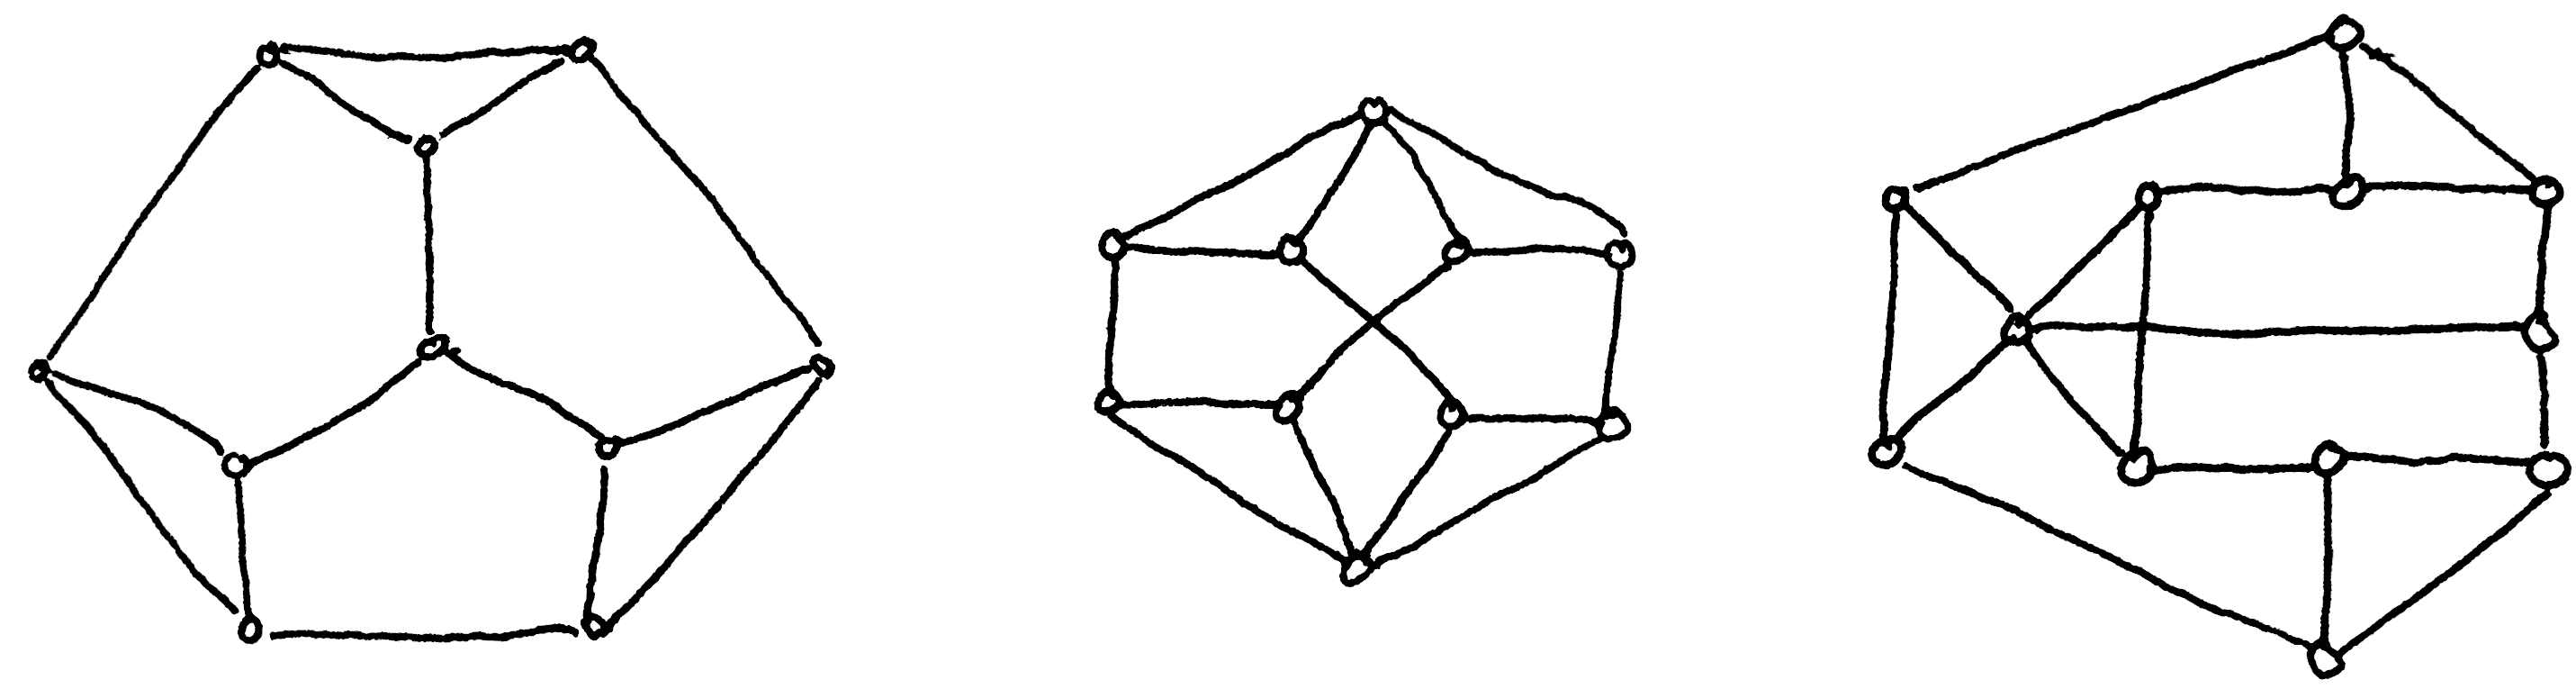
\includegraphics[width=120mm]{graphs/unemb-base-20.jpg}
    \end{center}
    which are unembeddable.  The left and middle graph
    are the only minimal unembeddable squarefree graph.
\end{comp}
For the first graph, we have proven directly that it is unembeddable.
See Proposition~\ref{prop:unemb-10-2}.
For the second graph, we also have a direct proof.

\section{Conclusion and future research}
TODO

\section{Acknowledgments}
We wish to thank the following for their generous contribution to the
distributed computation:
    the Digital Security group, Intelligent Systems group
    and the C\&CZ service of the Radboud University;
    Wouter Geraedts and
    Jille Timmermans.

We are grateful to prof.~McKay for discussing
the feasability of certain graph restrictions.

\appendix
\section{Example reduce script}\label{adx:unemb-10-2}
The following is (a part of) the reduce script mechanically generated
to prove the non-embeddability of the graph of Figure~\ref{fig:unemb-10-2}.
The algorithm choose a different assignment, than we did in the
proof of Proposition~\ref{prop:unemb-10-2}.
As free points it picked, in order,~$z$, $x$, $v$ and~$p_3$.
The point~$w$ is assigned~$p_3 \times z$.
\begin{verbatim}
load_package redlog;
rlset R;

procedure d(x,y);
    (first x) * (first y) +
    (second x) * (second y) +
    (third x) * (third y);

procedure k(x,y);
    {(second x)*(third y) - (third x)*(second y),
     (third x)*(first y) - (first x)*(third y),
     (first x)*(second y) - (second x)*(first y)};

v0c1 := 1; v0c2 := 0; v0c3 := 0;
v1c1 := 0; v1c2 := 1; v1c3 := 0;

v0 := {v0c1, v0c2, v0c3}; 
v1 := {v1c1, v1c2, v1c3}; 
v2 := {v2c1, v2c2, v2c3}; 
v3 := {v3c1, v3c2, v3c3}; 
v2c1 := 0;
neq0 := k(v0,k(v3,v1)); 
\end{verbatim}
\begin{center} \emph{(snip)} \end{center}
\begin{verbatim}
neq29 := k(k(k(k(v3,v1),v1),v2),k(k(v3,v0),v3)); 
phi := 
       (first neq0 neq 0 or
        second neq0 neq 0 or
        third neq0 neq 0) and 
\end{verbatim}
\begin{center} \emph{(snip)} \end{center}
\begin{verbatim}
       (first neq29 neq 0 or
        second neq29 neq 0 or
        third neq29 neq 0) and 
       d(v2,v0) = 0 and 
       d(k(k(v3,v0),v3),k(k(k(k(v3,v1),v1),v2),v2)) = 0 and 
        true;
rlqe ex(v3c3,
     ex(v3c2,
     ex(v3c1,
     ex(v2c3,
     ex(v2c2,phi)))));
\end{verbatim}


% attribute mckay for answering questions?
% TODO attribute geng
\bibliography{main}{}
\bibliographystyle{plain}


\end{document}

% vim: ft=tex.latex
